\section{Actions}

There are two parts to the action definition. One part defines an interface with OpenAI Gym to let interact with the agent. The other part is the environment, receiving the action and processing it further, such as cropping it and scaling it. An example of an action space definition is given below \ref{code:actdefine}. 

\begin{lstlisting}[language=Python, caption=OpenAI gym action space definition, label=code:actdefine]

    if not self._discrete:
        self.action_space = gym.spaces.Box(-1.,
                                             1., shape=(3,), dtype=np.float32)
    else:
        self.action_space = gym.spaces.Discrete(self.num_actions_pad*3)

\end{lstlisting}


It defines the action type and the shape of the action. This definition is later processed by the RL algorithm to output an action based on what the environment expects. Our environment takes only continuous actions. However, to try the DQN algorithm, which output only discrete, we linearly discretized the environment. Based on the discretization padding given in the configuration file, we define the size of the discrete action space. For instance, if the discretization padding is three for each action dimension, and if the simplified environment is set, we would have nine actions. Since the simplified environment has three actions dimension and three actions padding for each action makes up in a total of nine actions. The below diagram presents the linear action discretization \ref{fig:disc}.

\begin{figure}[htbp]
    \centering
    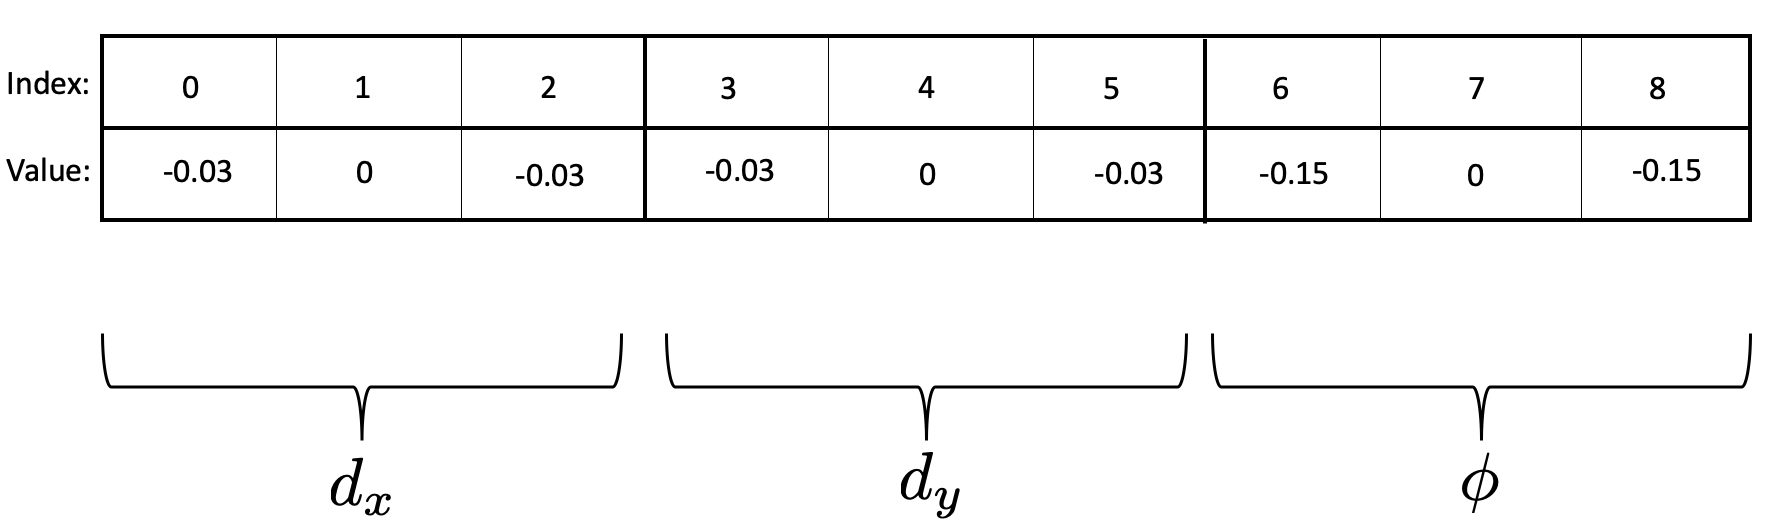
\includegraphics[width=1\textwidth]{figures/discretization.png}
    \caption{Linear action discretization representation. Padding one action dimenstion is 3 and total number of action dimension is 3}
    \label{fig:disc}
\end{figure}

As mentioned in Stable-Baselines documentation \footnote{\url{https://bit.ly/2PYe5hG}} continuous actions algorithms work best when the action space is defined symmetric and between -1 and 1. Therefore, we need to rescale the actions in the environment side to fit the maximum action limits. This problem does not appear on the discrete action space because we already receive the action index from the DQN algorithm and can easily assign it to the respective values.